\documentclass[11pt,a4paper]{article}
\usepackage[a4paper,hmargin=1in,vmargin=1in]{geometry}
\usepackage{pgfplots}
\pgfplotsset{compat=1.17}

\usepackage[czech]{babel}
\usepackage[utf8]{inputenc}
\usepackage[T1]{fontenc}

\usepackage[nodayofweek]{datetime}
\newdate{date}{15}{6}{2023}

\usepackage{stddoc}
\usepackage{lipsum}
\usepackage{subcaption}
% \usepackage[square,numbers]{natbib}
% \usepackage[nottoc]{tocbibind}

\newcommand{\plus}{{\texttt{+}}}
\renewcommand{\Re}{\operatorname{Re}}
\renewcommand{\Im}{\operatorname{Im}}
\newcommand{\fourier}[3]{\mathcal{F}_{#1}\!\left[#2\right]\!\left(#3\right)}
\newcommand{\ifourier}[3]{\mathcal{F}^{-1}_{#1}\!\left[#2\right]\!\left(#3\right)}
\newcommand{\Ohm}{\mathrm{\Omega}}
\newcommand{\dB}{\mathrm{dB}}
\newcommand{\dBm}{\mathrm{dBm}}
\newcommand{\MHz}{\mathrm{MHz}}
\newcommand{\GHz}{\mathrm{GHz}}
\newcommand{\kHz}{\mathrm{kHz}}


\begin{document}

\pagenumbering{arabic}

% Header
\begin{center}
    {\LARGE\textbf{Laboratorní úloha č. 10}}\\[3mm]
    \begin{minipage}{0.4\textwidth}
        \begin{flushleft}
            \textsc{\displaydate{date}}
        \end{flushleft}
    \end{minipage}
    ~
    \begin{minipage}{0.4\textwidth}
        \begin{flushright}
            \textsc{Martin Šimák}
        \end{flushright}
    \end{minipage}
    \noindent\rule{14.5cm}{0.4pt}
\end{center}

\paragraph*{Měření činitele jakosti Q rezonátorů} Laboratorní úloha ukazuje možnosti vektorového měření při určování jakosti rezonátorů a definování rovnic ve vektorovém analyzátoru.

\subsection*{Úkoly měření}
\begin{enumerate}
    \item Změřte pod vedením vyučujícího pomocí vektorového analyzátoru Agilent E8364A jednotlivé činitele jakosti \emph{dutinového}, \emph{mikropáskového} a \emph{dielektrického} rezonátoru a určete jejich náhradní obvody. U dielektrického rezonátoru proměřte vlastnosti jak bez odrazného terčíku, tak s odrazným terčíkem.
    \item V referenční rovině měření v místě vazby na rezonátor určete typ rezonančního obvodu a reálnou složku impedance či admitance. Dále určete potřebné frekvence dle metod popsaných v~\cite{tysl:mereni-pri-velmi-vysokych-kmitoctech},~\cite{khanna-garault:determination-of-q}~a~\cite{khanna:q-measurement-of-coupled-microstrips}.
    \item Z naměřených hodnot odvoďte náhradní obvod rezonančních obvodů a určete hodnoty jeho prvků.
\end{enumerate}

\subsection*{Použité přístroje a komponenty}
\begin{itemize}
    \item Vektorový analyzátor Agilent E8364A (45~MHz až 50~GHz)
\end{itemize}

\subsection*{Popis měření}
\paragraph*{Teoretický úvod} Při měření na VNA je naprosto nezbytné se vždy vyhnout elektrostatickému výboji na středním vodiči testovacích kabelů či na vodičích s nimi spojenými. Je proto nutno vyloučit dotyk ruky s těmito vodiči a používat zemněný náramek.

V rámci měření určujeme celkem tři činitele jakosti: \emph{nezatížený} činitel jakosti $Q_u$, \emph{zatížený} činitel jakosti $Q_L$ a \emph{externí} činitel jakosti $Q_{\mathrm{ext}}$. Mezi těmito činiteli platí relace
\begin{align*}
    Q_u = Q_L(1+\beta)=\beta Q_{\mathrm{ext}},
\end{align*}
kde $\beta$ je koeficient vazby rezonátoru na vedení. Jak pojednává článek~\cite{tysl:mereni-pri-velmi-vysokych-kmitoctech}, pro určení všech tří činitelů jakosti je nutné určit postupně frekvence $f_1$ a $f_2$, kdy platí rovnost $\Re(Z) = \pm\Im(Z)$; frekvence $f_3$ a $f_4$, kdy $\Im(Z) = \pm(\Re(Z) + 50\ \Ohm)$; frekvence $f_5$ a $f_6$, kdy $\Im(Z) = \pm1$. Všechny tyto významné frekvence jsou ilustrovány na obrázku~\ref{fig:smitak-kruznice} a pro činitele jakosti potom platí
\begin{align}
    Q_u &= \frac{f_0}{f_1-f_2},
    &
    Q_L &= \frac{f_0}{f_3-f_4},
    &
    Q_{\mathrm{ext}} &= \frac{f_0}{f_5-f_6},
\end{align}
kde $f_0$ je rezonanční frekvence.
\begin{figure}[!ht]
    \centering
    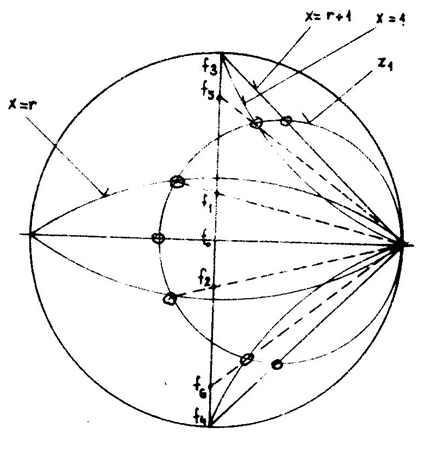
\includegraphics[width=.5\textwidth]{src/smitak-kruznice.png}
    \caption{\label{fig:smitak-kruznice}Vyznamné frekvenční body pro výpočet činitelů jakosti}
\end{figure}

Za znalosti nezatíženého činitele jakosti $Q_u$ lze spočítat kapacitu kondenzátoru a indukčnost cívky v náhradním obvodu rezonátoru. V případě paralelní rezonance platí vztah
\begin{align}
    Q_u = 2\pi f_0RC,
\end{align}
zatímco pro sériovou rezonanci platí
\begin{align}
    Q_u = \frac{2\pi f_0 L}{R}.
\end{align}
Hodnotu druhého reaktančního prvku vždy určíme z Thomsonova vztahu pro rezonanci ve tvaru
\begin{align}
    f_0 = \frac{1}{2\pi\sqrt{LC}}.
\end{align}

% Task 1
\paragraph*{Měření dutinového rezonátoru} Před měřením jakosti dutinového rezonátoru je nutné nejprve zkalibrovat VNA na dané měření -- v našem případě metodou TRL na vlnovodu R100. Dále abychom se vyhnuli potenciálnímu vynechání ostré rezonance, je vhodné nastavit vysoký počet frekvenčních bodů (16001). Frekvenční pásmo je 8~GHz až 12.4~GHz, což můžeme dále zúžit na okolí rezonanční frekvence tak, abychom mohli jemně posouvat kurzor po rezonanční křivce Smithova diagramu. Případně lze i zmenšit počet frekvenčních bodů.

\subparagraph*{Výsledky měření} Během měření jsme pozorovali smyčku paralelní rezonance s odporem v rezonanci $R = 15.6\ \Ohm$. Naměřené hodnoty frekvencí významných pro určení činitelů jakosti jsou zaneseny v tabulce~\ref{table:dutinovy-rezonator-frekvence}. Z těchto dat jsou vypočtené hodnoty parametrů náhradního obvodového zapojení rezonátoru v tabulce~\ref{table:dutinovy-rezonator-hodnoty}.
\begin{table}[!ht]
\centering
\begin{tabular}{|c|c|c|c|c|c|c|}
    \hline
    $f_0\ [\GHz]$ & $f_1\ [\GHz]$ & $f_2\ [\GHz]$ & $f_3\ [\GHz]$ & $f_4\ [\GHz]$ & $f_5\ [\GHz]$ & $f_6\ [\GHz]$\\
    \hline\hline
    10.27493 & 10.27526 & 10.27458 & 10.27536 & 10.27446 & 10.27502 & 10.27480\\
    \hline
\end{tabular}
\caption{\label{table:dutinovy-rezonator-frekvence}Vyznamné frekvence pro dutinový rezonátor}
\end{table}
\begin{table}[!ht]
\centering
\begin{tabular}{|c|c|c|c|c|c|}
    \hline
    $Q_u\ [-]$ & $Q_L\ [-]$ & $Q_{\mathrm{ext}}\ [-]$ & $R\ [\mathrm{\Omega}]$ & $C\ [\mathrm{nF}]$ & $L\ [\mathrm{fH}$]\\
    \hline\hline
    15110 & 11417 & 46704 & 15.6 & 15.0 & 16\\
    \hline
\end{tabular}
\caption{\label{table:dutinovy-rezonator-hodnoty}Činitelé jakosti a parametry náhradního obvodu dutinového rezonátoru}
\end{table}

% Task 2
\paragraph*{Měření mikropáskového rezonátoru} Pro měření na mikropáskovém vedení kalibrujeme VNA na konci testovacích kabelů pomocí metody OSM. Použitý kalibrační kit je Agilent 85052C 3.5~mm Precision Calibration Kit. Počet frekvenčních bodů je vhodné opět navýšit na 16001 a frekvenční pásmo je 1~GHz až 18~GHz. Po připojení přípravku s mikropáskových rezonátorem vybereme vhodnou rezonanční smyčku%
    \footnote{Rezonanční smyčky lze odlišit od zbytku chování obvodu zatlumením rezonátoru dotykem prstu. Dotyku s vazebním mikropáskem bychom se však měli vyvarovat.}
a nastavíme užší frekvenční pásmo pokrývající její nejbližší okolí. Dále je vhodné při zatlumeném rezonátoru pomocí nastavení \emph{Scale/Electrical Delay} nastavit referenční rovinu měření na konec vazebního mikropáskového vedení. Po odtlumení již lze rozpoznat typ rezonančního obvodu, na základě čehož můžeme postupovat dle~\cite{tysl:mereni-pri-velmi-vysokych-kmitoctech}, tj. posunout rezonanční smyčku symetricky kolem imaginární osy, určit rezonanční odpor a výsledně získat pomocí uvedených vztahů jednotlivé činitele jakosti.

\subparagraph*{Výsledky měření} Během měření jsme pozorovali smyčku sériové rezonance s odporem v rezonanci $R = 32.2\ \Ohm$. Naměřené hodnoty frekvencí významných pro určení činitelů jakosti jsou zaneseny v tabulce~\ref{table:mikropaskovy-rezonator-frekvence}. Z těchto dat jsou vypočtené hodnoty parametrů náhradního obvodového zapojení rezonátoru v tabulce~\ref{table:mikropaskovy-rezonator-hodnoty}.
\begin{table}[!ht]
\centering
\begin{tabular}{|c|c|c|c|c|c|c|}
    \hline
    $f_0\ [\GHz]$ & $f_1\ [\GHz]$ & $f_2\ [\GHz]$ & $f_3\ [\GHz]$ & $f_4\ [\GHz]$ & $f_5\ [\GHz]$ & $f_6\ [\GHz]$\\
    \hline\hline
    10.36582 & 10.38422 & 10.34782 & 10.41062 & 10.32462 & 10.39342 & 10.33982\\
    \hline
\end{tabular}
\caption{\label{table:mikropaskovy-rezonator-frekvence}Vyznamné frekvence pro mikropáskový rezonátor}
\end{table}
\begin{table}[!ht]
\centering
\begin{tabular}{|c|c|c|c|c|c|}
    \hline
    $Q_u\ [-]$ & $Q_L\ [-]$ & $Q_{\mathrm{ext}}\ [-]$ & $R\ [\mathrm{\Omega}]$ & $C\ [\mathrm{fF}]$ & $L\ [\mathrm{nH}$]\\
    \hline\hline
    285 & 121 & 193 & 32.2 & 1.7 & 140.9\\
    \hline
\end{tabular}
\caption{\label{table:mikropaskovy-rezonator-hodnoty}Činitelé jakosti a parametry náhradního obvodu mikropáskového rezonátoru}
\end{table}

% Task 3
\paragraph*{Určení typu rezonančnho obvodu dielektrického rezonátoru} Dielektrický rezonátor měříme navázaný na bezodrazově zakončené mikropáskové vedení. Nejprve je třeba rozšířit frekvenční pásmo na 8~GHz až 12~GHz, kde lze očekávat rezonanční frekvenci rezonátoru. Dále odpojííme výstupní adaptér s $50\Ohm$ zátěží a nastavíme frekvenční rovinu měření na konec mikropásku pomocí nastavení \emph{Scale/Electrical Delay}. Následně zmenšíme \emph{Electrical delay} tak, aby sbalené klubíčko a tím i referenční rovina byla v místě zkratu. Potřebnou hodnotu \emph{Electrical delay} si poznamenáme. Do této referenční roviny, která je $\lambda/4$ od otevřeného konce a která je bodem maxima magnetického pole, umístíme dielektrický rezonátor. Z charakteru rezonanční smyčku lze určit typ rezonančního obvodu.

\subparagraph*{Výsledky měření} Během měření jsme pozorovali smyčku paralelní rezonance.

% Task 4
\paragraph*{Určení vlastností dielektrického rezonátoru} Tento úkol přímo na navazuje na předchozí s tím, že připojíme zpět výstupní adaptér $50\Ohm$ zátěže k přípravku a odpojíme vstupní adaptér SMA-mikropásek spolu s testovacím kabelem. Pomocí zvětšení hodnoty \emph{Scale/Electrical Delay} o poznamenanou hodnotu posuneme referenční rovinu o $\lambda/4$ dovnitř mikropásku. V této referenční rovině pak umišťujeme dielektrický rezonátor. Mechanickým přemístněním nebo jemnou změnou \emph{Electrical delay} nastavíme smyčku tak, aby byla symetrická vzhledem k imaginární ose.

Dle metody popsané v článcích~\cite{khanna-garault:determination-of-q}~a~\cite{khanna:q-measurement-of-coupled-microstrips} je nyní třeba smyčku $2\times$ zvětšit a posunout o hodnotu~$-1$. Dále určíme reálnou složku impedance na rezonanční frekvenci v impedančním Smithově diagramu pomocí markerů. Určená impdance odpovídá sériovému rezonančnímu odporu rezonátoru a $50\Ohm$ zátěže. Nyní již můžeme přepnout zobrazení do admitančního Smithova diagramu a odečíst hodnoty významných frekvencí pro určení činitelů jakosti.

\subparagraph*{Výsledky měření s terčíkem} Během měření jsme pozorovali smyčku paralelní rezonance s odporem v rezonanci $R = 461\ \Ohm$. Naměřené hodnoty frekvencí významných pro určení činitelů jakosti jsou zaneseny v tabulce~\ref{table:dielektricky-rezonator-s-tercikem-frekvence}. Z těchto dat jsou vypočtené hodnoty parametrů náhradního obvodového zapojení rezonátoru v tabulce~\ref{table:dielektricky-rezonator-s-tercikem-hodnoty}.
\begin{table}[!ht]
\centering
\begin{tabular}{|c|c|c|c|c|c|c|}
    \hline
    $f_0\ [\GHz]$ & $f_1\ [\GHz]$ & $f_2\ [\GHz]$ & $f_3\ [\GHz]$ & $f_4\ [\GHz]$ & $f_5\ [\GHz]$ & $f_6\ [\GHz]$\\
    \hline\hline
    10.4788 & 10.4680 & 10.4600 & 10.4885 & 10.4395 & 10.4830 & 10.4445\\
    \hline
\end{tabular}
\caption{\label{table:dielektricky-rezonator-s-tercikem-frekvence}Vyznamné frekvence pro dielektrický rezonátor s terčíkem}
\end{table}
\begin{table}[!ht]
\centering
\begin{tabular}{|c|c|c|c|c|c|}
    \hline
    $Q_u\ [-]$ & $Q_L\ [-]$ & $Q_{\mathrm{ext}}\ [-]$ & $R\ [\mathrm{\Omega}]$ & $C\ [\mathrm{pF}]$ & $L\ [\mathrm{pH}$]\\
    \hline\hline
    1310 & 213 & 272 & 461 & 43.2 & 5.3\\
    \hline
\end{tabular}
\caption{\label{table:dielektricky-rezonator-s-tercikem-hodnoty}Činitelé jakosti a parametry náhradního obvodu dielektrického rezonátoru s terčíkem}
\end{table}

\subparagraph*{Výsledky měření bez terčíku} Během měření jsme pozorovali smyčku paralelní rezonance s odporem v rezonanci $R = 183\ \Ohm$. Naměřené hodnoty frekvencí významných pro určení činitelů jakosti jsou zaneseny v tabulce~\ref{table:dielektricky-rezonator-bez-terciku-frekvence}. Z těchto dat jsou vypočtené hodnoty parametrů náhradního obvodového zapojení rezonátoru v tabulce~\ref{table:dielektricky-rezonator-bez-terciku-hodnoty}.
\begin{table}[!ht]
\centering
\begin{tabular}{|c|c|c|c|c|c|c|}
    \hline
    $f_0\ [\GHz]$ & $f_1\ [\GHz]$ & $f_2\ [\GHz]$ & $f_3\ [\GHz]$ & $f_4\ [\GHz]$ & $f_5\ [\GHz]$ & $f_6\ [\GHz]$\\
    \hline\hline
    10.3908 & 10.4100 & 10.3775 & 10.4325 & 10.3560 & 10.4135 & 10.3720\\
    \hline
\end{tabular}
\caption{\label{table:dielektricky-rezonator-bez-terciku-frekvence}Vyznamné frekvence pro dielektrický rezonátor bez terčíku}
\end{table}
\begin{table}[!ht]
\centering
\begin{tabular}{|c|c|c|c|c|c|}
    \hline
    $Q_u\ [-]$ & $Q_L\ [-]$ & $Q_{\mathrm{ext}}\ [-]$ & $R\ [\mathrm{\Omega}]$ & $C\ [\mathrm{pF}]$ & $L\ [\mathrm{pH}$]\\
    \hline\hline
    320 & 136 & 250 & 183 & 26.8 & 8.8\\
    \hline
\end{tabular}
\caption{\label{table:dielektricky-rezonator-bez-terciku-hodnoty}Činitelé jakosti a parametry náhradního obvodu dielektrického rezonátoru bez terčíku}
\end{table}

\subsection*{Závěr}
V rámci laboratorní úlohy jsme se seznámili s možnostmi vektorového měření při určování jakosti rezonátorů a definování rovnic ve vektorovém analyzátoru. K určení jednotlivých činitelů jakosti a parametrů náhradního obvodového zapojení měřených rezonátorů jsme využívali metod, které jsou popsány v odkazované literatuře a využvají impedančního měření. Měření proběhlo bez větších potíží a byli jsme tak schopni vyhodnotit a srovnat jakost jednotlivých rezonátorů. Jako nejkvalitnější se z hlediska činitelů jakosti jednoznačně jeví dutinový rezonátor, jehož hodnoty jsou mnohem vyšší než u ostatních typů.

\begin{thebibliography}{3}
    \bibitem{tysl:mereni-pri-velmi-vysokych-kmitoctech} Tysl V., \emph{Měření při velmi vysokých kmitočtech}, skriptum ČVUT FEL, listopad 1976, str. 90--96.
    
    \bibitem{khanna-garault:determination-of-q} Khanna A. P. S., Garault Y., \emph{Determination of Loaded, Unloaded, and External Quality Factors of a Dielectric Resonator Coupled to a Microstrip Line}, IEEE Trans. on MTT, vol. MTT-31, č. 3, březen 1983, str. 261--264.
    
    \bibitem{khanna:q-measurement-of-coupled-microstrips} Khanna A. P. S., \emph{Q measurement of microstrip coupled dielectric resonators}, Microwaves \& RF, leden 1984, str. 81--86.
\end{thebibliography}

\end{document}
